\documentclass[11pt,a4paper,oneside]{article}

% ── Encodage & Typographie ───────────────────────────────────────────────────
\usepackage[utf8]{inputenc}
\usepackage[T1]{fontenc}
\usepackage[french]{babel}
\usepackage{lmodern}
\usepackage{microtype}

% ── Marges & Mise en Page (Calibré pour 10 à 11 pages strictes) ──────────────
\usepackage[top=2.0cm, bottom=2.0cm, left=2.0cm, right=2.0cm, headheight=14pt, headsep=12pt]{geometry}
\usepackage{setspace}
\setstretch{1.22}

% ── Chemins Graphiques & Figures ──────────────────────────────────────────────
\usepackage{graphicx}
\graphicspath{{images/}{docs/images/}{../cyberscore-probe-agent/docs/images/}{assets/}{./}}
\usepackage[font=small,labelfont=bf,skip=5pt]{caption}

% ── Couleurs Institutionnelles TEK-UP & SOC ───────────────────────────────────
\usepackage{xcolor}
\definecolor{tekupPurple}{RGB}{74, 21, 110}  % Violet TEK-UP
\definecolor{tekupBlue}{RGB}{37, 99, 235}    % Bleu tech
\definecolor{socNavy}{RGB}{15, 23, 42}       % Ardoise sombre
\definecolor{socRed}{RGB}{220, 38, 38}       % Rouge alerte / ANCS
\definecolor{socGreen}{RGB}{16, 185, 129}    % Vert succès
\definecolor{codeBg}{RGB}{248, 250, 252}     % Fond code gris clair

% ── Tableaux, Boîtes & Graphiques ─────────────────────────────────────────────
\usepackage{tcolorbox}
\tcbuselibrary{skins,breakable}
\usepackage{tabularx}
\usepackage{booktabs}
\usepackage{array}
\usepackage{amsmath, amssymb}
\usepackage{enumitem}
\setlist[itemize]{noitemsep, topsep=2pt, parsep=0pt, leftmargin=15pt}
\setlist[enumerate]{noitemsep, topsep=2pt, parsep=0pt, leftmargin=15pt}

% ── Liens Hypertextes ─────────────────────────────────────────────────────────
\usepackage{hyperref}
\hypersetup{
    colorlinks=true,
    linkcolor=tekupPurple,
    citecolor=tekupBlue,
    urlcolor=tekupBlue
}

% ── En-têtes & Pieds de Page (fancyhdr) ───────────────────────────────────────
\usepackage{fancyhdr}
\pagestyle{fancy}
\fancyhf{}
\fancyhead[L]{\footnotesize \textcolor{tekupPurple}{\textbf{CyberScore TN -- Probe Agent}} \textbar{} Rapport Technique Scan Actif}
\fancyhead[R]{\footnotesize \textit{TEK-UP University}}
\fancyfoot[L]{\footnotesize \color{gray} Yosri HAMDOUNI \& Wajdi HAMDI -- PFA Cybersécurité}
\fancyfoot[R]{\thepage}
\renewcommand{\headrulewidth}{0.4pt}
\renewcommand{\footrulewidth}{0.4pt}

% ── Formatage des Sections ───────────────────────────────────────────────────
\usepackage{titlesec}
\titleformat{\section}
    {\normalfont\Large\bfseries\color{tekupPurple}}
    {\thesection.}{7pt}{\Large}
\titleformat{\subsection}
    {\normalfont\large\bfseries\color{socNavy}}
    {\thesubsection.}{5pt}{\large}
\titlespacing*{\section}{0pt}{9pt plus 2pt minus 1pt}{4pt plus 1pt minus 1pt}
\titlespacing*{\subsection}{0pt}{6pt plus 1pt minus 1pt}{3pt plus 1pt minus 1pt}

% ── Configuration des Extraits de Code ───────────────────────────────────────
\usepackage{listings}
\lstset{
    backgroundcolor=\color{codeBg},
    basicstyle=\ttfamily\footnotesize,
    keywordstyle=\color{tekupPurple}\bfseries,
    commentstyle=\color{gray}\itshape,
    stringstyle=\color{tekupBlue},
    numbers=none,
    frame=single,
    rulecolor=\color{gray!30},
    breaklines=true,
    captionpos=b
}

\begin{document}

% ==============================================================================
% PAGE DE GARDE OFFICIELLE
% ==============================================================================
\begin{titlepage}
\begin{center}

% En-tête Logos ou Mentions
\begin{minipage}[c]{0.35\textwidth}
    \flushleft
    \IfFileExists{images/logo_tekup.png}{%
        
\includegraphics[height=1.9cm]{images/logo_tekup.png}%
    }{%
        \IfFileExists{logo_tekup.png}{%
            
\includegraphics[height=1.9cm]{logo_tekup.png}%
        }{\textbf{\large TEK-UP University}}%
    }
\end{minipage}
\hfill
\begin{minipage}[c]{0.28\textwidth}
    \centering
    \scriptsize
    \textbf{RÉPUBLIQUE TUNISIENNE}\\[1mm]
    \tiny
    Ministère de l'Enseignement Supérieur\\
    et de la Recherche Scientifique
\end{minipage}
\hfill
\begin{minipage}[c]{0.35\textwidth}
    \flushright
    \IfFileExists{images/logo_ancs.png}{%
        
\includegraphics[height=1.9cm]{images/logo_ancs.png}%
    }{%
        \IfFileExists{logo_ancs.png}{%
            
\includegraphics[height=1.9cm]{logo_ancs.png}%
        }{\textbf{\large ANCS Tunisie}}%
    }
\end{minipage}

\vspace{0.7cm}

{\large \textbf{TEK-UP UNIVERSITY}}\\[1.5mm]
{\small \textbf{ÉCOLE SUPÉRIEURE PRIVÉE DE TECHNOLOGIES ET D'INGÉNIERIE}}\\[1mm]
{\footnotesize Département Génie Informatique \& Cybersécurité}\\[2.5mm]
{\color{tekupPurple}\rule{0.85\textwidth}{1.5pt}}

\vspace{0.7cm}

{\large \textbf{RAPPORT DE PROJET DE FIN D'ANNÉE (PFA)}}\\[1.5mm]
{\footnotesize Présenté en vue de l'obtention du}\\[1.5mm]
{\large \textbf{DIPLÔME NATIONAL D'INGÉNIEUR EN GÉNIE INFORMATIQUE}}\\[1mm]
{\small \textit{Spécialité : Cybersécurité \& Systèmes Distribués}}

\vspace{0.8cm}

% Cadre Titre
\begin{tcolorbox}[
    colback=white,
    colframe=tekupPurple,
    arc=1mm,
    boxrule=1.5pt,
    left=12pt,
    right=12pt,
    top=9pt,
    bottom=9pt
]
    \centering
    {\huge \bfseries \color{tekupPurple} CyberScore TN -- Probe Agent}\\[2.5mm]
    {\large \textbf{Conception et Déploiement d'un Moteur d'Audit Actif Autonome Multi-Agents et d'une Infrastructure Souveraine Cloisonnée}}
\end{tcolorbox}

\vspace{0.9cm}

% Binôme & Partenaire
\begin{minipage}[t]{0.48\textwidth}
    \flushleft
    \textbf{Élaboré par :}\\[2mm]
    {\large \textbf{Yosri HAMDOUNI}}\\[1mm]
    {\large \textbf{Wajdi HAMDI}}\\[2.5mm]
    \footnotesize \textit{Élèves Ingénieurs en Cybersécurité}
\end{minipage}
\hfill
\begin{minipage}[t]{0.48\textwidth}
    \flushleft
    \textbf{Organisme Partenaire :}\\[2mm]
    {\textbf{ANCS} (Agence Nationale de la Cybersécurité)}\\[1.5mm]
    \footnotesize \textit{Cadre légal : Décret-loi n° 2023-17}\\[2mm]
    \textbf{Session Universitaire :}\\[1mm]
    {\small Année Académique 2025 -- 2026}
\end{minipage}

\vfill

{\footnotesize Tunis, Tunisie -- Juin 2026}

\end{center}
\end{titlepage}

% ==============================================================================
% SOMMAIRE EXÉCUTIF
% ==============================================================================
\tableofcontents
\newpage

% ==============================================================================
% 1. INTRODUCTION GÉNÉRALE & CONTEXTE
% ==============================================================================
\section{Introduction Générale \& Contexte Académique}

Dans le cadre de notre projet de fin d'année d'ingénieur à TEK-UP, nous nous sommes intéressés à la sécurisation offensive éthique des infrastructures numériques de l'État tunisien. En complément de la plateforme d'audit passif \textbf{CyberScore TN}, qui analyse l'empreinte externe publique des portails étatiques (\texttt{.gov.tn}, \texttt{.tn} souverains), nous avons conçu et déployé \textbf{Probe Agent} : un moteur d'audit actif autonome multi-agents.

\subsection{Problématique des Scanners Conventionnels}
Dans la pratique industrielle, les scanners de vulnérabilités traditionnels (tels que Nessus, OpenVAS ou Acunetix) présentent des limites structurelles majeures lorsqu'ils sont confrontés à des parcs ministériels sensibles :
\begin{enumerate}
    \item \textbf{Le fléau des faux positifs :} En se fondant quasi-exclusivement sur la lecture statique des bannières applicatives (par exemple \textit{Apache 2.4.41}), ces outils déclarent des dizaines de CVE critiques qui ne sont en réalité pas exploitables (modules désactivés, pare-feu WAF en coupure). Les équipes de sécurité se retrouvent paralysées face à des alertes erronées.
    \item \textbf{Le risque de déni de service (DoS) :} Les rafales agressives et non modulées peuvent saturer ou faire tomber des serveurs administratifs à faible tolérance de charge.
    \item \textbf{La dépendance envers des clouds tiers :} L'envoi de télémétrie et d'empreintes techniques vers des infrastructures d'inférence étrangères contrevient aux principes de souveraineté nationale et au secret d'État.
\end{enumerate}

\subsection{Objectifs du Projet Académique}
Notre travail d'ingénierie vise à résoudre cette triple contrainte à travers :
\begin{itemize}
    \item L'orchestration d'un \textbf{pipeline séquentiel de 4 agents logiciels coopératifs} en Python asynchrone.
    \item L'application rigoureuse de la doctrine du \textbf{Zéro Faux Positif} via des preuves de concept (PoC) dynamiques et non destructives.
    \item L'intégration d'un modèle d'\textbf{IA souverain 100\% local} (Ollama Qwen2.5-Coder:7B) pour l'assistance contextuelle déterministe.
    \item Le confinement de la sonde au sein d'une \textbf{architecture Tri-VM} isolée, sous domaine unifié \texttt{cyberscore.tn} et durcie sous RHEL 9.5 (SELinux Enforcing).
\end{itemize}

% ==============================================================================
% 2. CADRAGE RÉGLEMENTAIRE & DOCTRINE ZÉRO FAUX POSITIF
% ==============================================================================
\section{Cadrage Réglementaire \& Doctrine « Zéro Faux Positif »}

\subsection{Distinction Fondamentale : Passif vs Actif}
Un audit de sécurité ne peut être conduit sans délimiter avec précision la frontière entre observation extérieure et interaction réseau :

\begin{table}[htbp]
\centering
\small
\renewcommand{\arraystretch}{1.1}
\begin{tabularx}{\textwidth}{lXX}
\toprule
\textbf{Critère} & \textbf{Audit Passif (16 Piliers OSINT)} & \textbf{Audit Actif (Probe Agent)} \\
\midrule
\textbf{Interaction réseau} & Consultation DNS, certificats TLS, en-têtes HTTP & Paquets TCP SYN ciblés, sondes de test HTTP \\
\textbf{Impact cible} & Strictement nul (zéro sollicitation réseau) & Trafic contrôlé, borné et temporisé ($<$ 800 ms) \\
\textbf{Exigence légale} & Accès libre (sources ouvertes OSINT) & \textbf{Mandat officiel obligatoire} (Décret 2023-17) \\
\textbf{Profil requis} & Consultation publique & Auditeur habilité / Officier certifié ANCS \\
\bottomrule
\end{tabularx}
\caption{Comparaison fonctionnelle et juridique entre audit passif et actif}
\end{table}

\subsection{Règles d'Engagement (RoE) \& Décret ANCS 2023-17}
Conformément au Décret-loi n° 2023-17 du 11 mars 2023 relatif à la cybersécurité, aucun tir actif ne peut débuter sans que trois verrous stricts ne soient validés par la passerelle applicative :
\begin{itemize}
    \item \textbf{Mandat d'audit vérifié :} Saisie obligatoire d'un identifiant de mandat officiel valide (\texttt{ANCS-2026}, \texttt{ANCS-SEC-2026}, \texttt{ANCS-VAL-2026}).
    \item \textbf{Périmètre d'attribution strict :} Vérification systématique de l'appartenance de l'IP cible au réseau souverain tunisien (AS2609 de l'ATI, préfixes \texttt{193.95.*}, \texttt{41.22.*}), interdisant formellement tout tir vers une cible tierce ou étrangère.
    \item \textbf{Classification TLP:AMBER :} Les résultats d'audit sont cryptographiquement signés et soumis à diffusion restreinte avec traçabilité de la signature numérique de l'auditeur.
\end{itemize}

\subsection{La Règle Cardinale du Zéro Faux Positif}
La doctrine cardinale de notre moteur stipule qu'\textit{une vulnérabilité théorique ne peut être imputée à un serveur si sa faisabilité pratique n'a pas été formellement démontrée}. Dès lors, une faille n'est certifiée que si une sonde d'expérimentation inoffensive (PoC bénin) produit une réponse anormale confirmant l'exploitabilité. Si le test est bloqué par un WAF ou inopérant, la vulnérabilité est rejetée du rapport officiel.

% ==============================================================================
% 3. ARCHITECTURE DU SYSTÈME & INFRASTRUCTURE TRI-VM
% ==============================================================================
\section{Architecture Globale \& Infrastructure Tri-VM Cloisonnée}

Afin de satisfaire aux exigences de haute disponibilité, de sécurité offensive et d'isolation des responsabilités, la solution repose sur une architecture découplée organisée en 6 tiers distincts.

\begin{figure}[htbp]
\centering
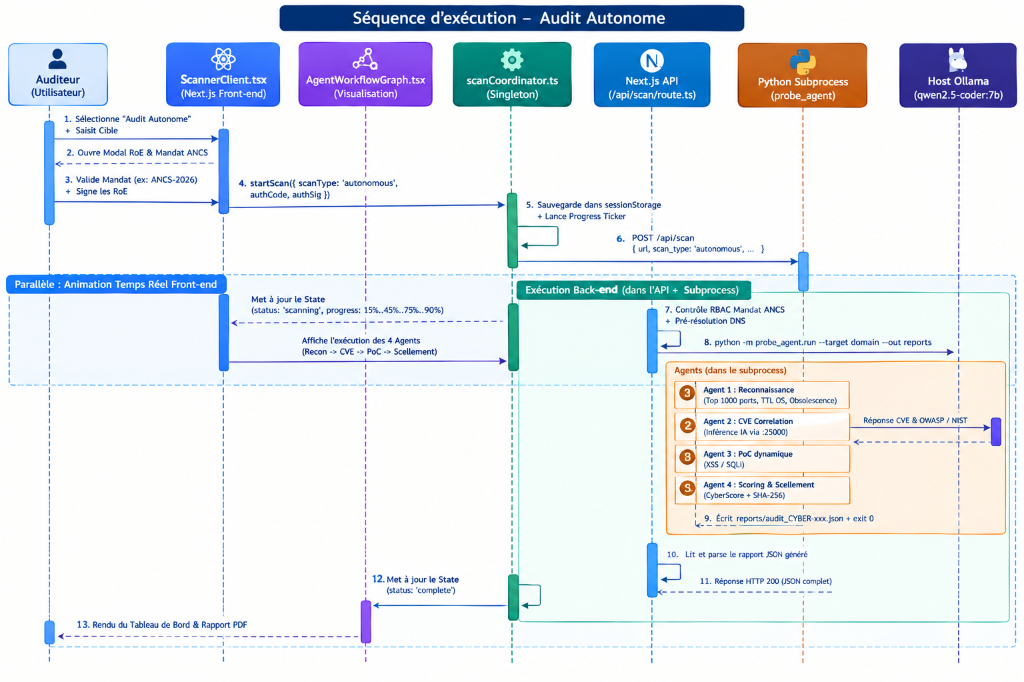
\includegraphics[width=0.74\textwidth]{architecture.png}
\caption{Architecture globale en 6 tiers et infrastructure réseau du Probe Agent}
\end{figure}

\subsection{Décomposition en 6 Tiers Découplés}
L'architecture de la sonde s'articule autour des couches opérationnelles suivantes :
\begin{enumerate}
    \item \textbf{Tier 1 : Frontend UI \& State (Next.js 14 App Router) :} Composants \texttt{ScannerClient.tsx} et \texttt{AgentWorkflowGraph.tsx}. Il gère l'affichage dynamique, le modal RoE et la persistance de session via un singleton mémoire (\texttt{scanCoordinator.ts}).
    \item \textbf{Tier 2 : API Gatekeeper \& RBAC (\texttt{route.ts}) :} Valide les accréditations ANCS, résout le DNS, contrôle les plages IP ATI (AS2609), et lance le sous-processus Python isolé avec un timeout strict de 240 secondes.
    \item \textbf{Tier 3 : Audit Bastion Sandbox (VM 3) :} Environnement d'exécution confiné sous RHEL 9.5 Minimal hébergeant les 4 agents d'audit.
    \item \textbf{Tier 4 : Multi-Agent Pipeline (\texttt{PentestOrchestrator}) :} Moteur asynchrone orchestrant l'état partagé \texttt{AuditState} à travers les 4 agents coopératifs.
    \item \textbf{Tier 5 : Inférence IA Locale Souveraine (Ollama Qwen2.5-Coder:7B) :} Nœud d'IA local interrogé en REST (port 25000), garantissant un traitement sans aucune fuite vers le cloud.
    \item \textbf{Tier 6 : Delivery \& Cryptographic Integrity :} Générateur de rapports JSON et attestations PDF certifiées avec sceau SHA-256 et QR Code de vérification publique.
\end{enumerate}

\subsection{Matrice de Répartition Tri-VM}
L'infrastructure physique et virtualisée sépare strictement les rôles pour éviter toute contamination :

\begin{table}[htbp]
\centering
\small
\renewcommand{\arraystretch}{1.1}
\begin{tabularx}{\textwidth}{llllX}
\toprule
\textbf{VM} & \textbf{Rôle} & \textbf{Adresse IP} & \textbf{Port exposé} & \textbf{Composants hébergés} \\
\midrule
\textbf{VM 1} & Frontend Public & \texttt{192.168.98.150} & 443 (HTTPS) & Next.js 14, Nginx Reverse Proxy, TLS Terminaison \\
\textbf{VM 2} & Backend \& IA & \texttt{192.168.98.149} & 8000 / 25000 & FastAPI, PostgreSQL, Redis, Ollama (Qwen 7B) \\
\textbf{VM 3} & Bastion Probe & \texttt{192.168.98.148} & Réseau privé & Probe Agent (4 Agents Python), Scapy, Socket raw \\
\bottomrule
\end{tabularx}
\caption{Matrice d'allocation des machines virtuelles et cloisonnement des services}
\end{table}

\subsection{Confinement \& Durcissement du Bastion (VM 3)}
L'externalisation du moteur d'audit sur une VM dédiée constitue un choix de sécurité stratégique :
\begin{itemize}
    \item \textbf{SELinux en mode Enforcing :} Verrouille strictement les capacités du processus Python, interdisant toute modification des binaires système.
    \item \textbf{Politique Firewalld par défaut à DROP :} Seules les requêtes sortantes de sondage et les communications internes autorisées sont admises.
    \item \textbf{Résilience face aux mécanismes défensifs :} Si l'adresse IP de la sonde est bannie par un Fail2ban ou un IDS/IPS cible, le portail web public (\texttt{VM 1}) et l'accès des usagers restent 100\% opérationnels.
    \item \textbf{Empreinte mémoire ultra-réduite :} L'ensemble du moteur de scan consomme moins de 50~Mo de mémoire vive au repos et moins de 180~Mo en plein tir.
\end{itemize}

% ==============================================================================
% 4. FONCTIONNEMENT DÉTAILLÉ DU PIPELINE MULTI-AGENTS
% ==============================================================================
\section{Fonctionnement Détaillé du Pipeline à 4 Agents Coopératifs}

Le cœur de l'audit actif est piloté par la classe \texttt{PentestOrchestrator}. Les agents coopèrent séquentiellement via la structure partagée \texttt{AuditState}.

\begin{figure}[htbp]
\centering
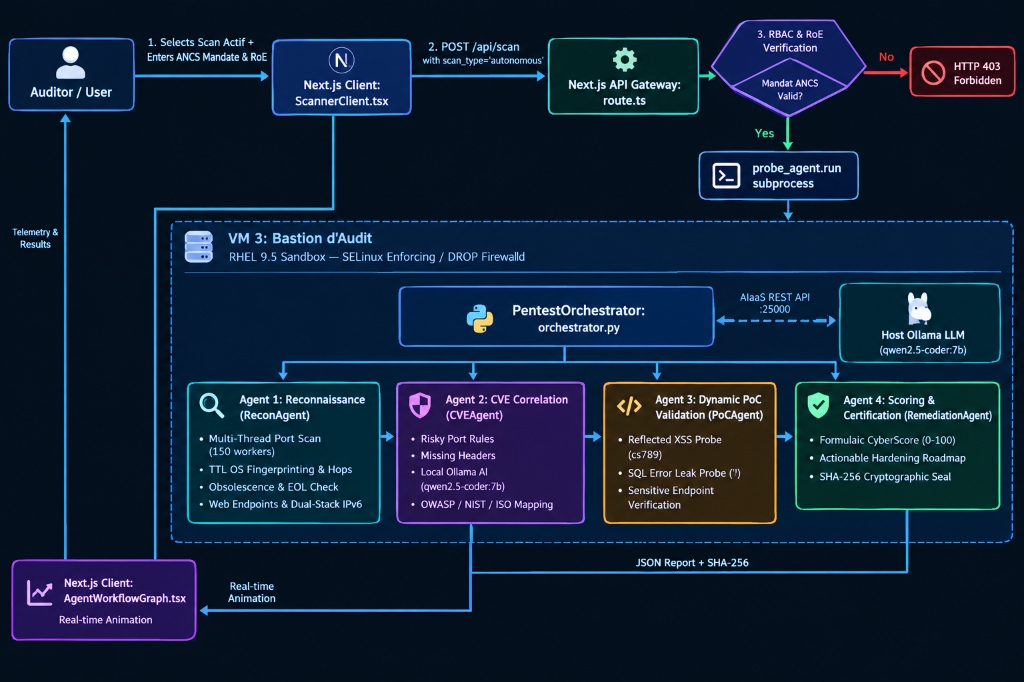
\includegraphics[width=0.74\textwidth]{execution_sequence.jpg}
\caption{Diagramme de séquence de l'exécution complète de l'audit actif autonome}
\end{figure}

\subsection{Agent 1 : Cartographie Avancée \& Reconnaissance (0\% -- 25\%)}
L'Agent 1 (\texttt{recon\_agent.py}) dresse la cartographie complète de la surface d'attaque en préservant l'intégrité de la cible :
\begin{itemize}
    \item \textbf{Scan de ports multithreadé haute vitesse (\texttt{port\_scanner.py}) :} Déployé avec un pool de \textbf{150 threads concurrents} (\texttt{ThreadPoolExecutor}) balayant le Top 1000 ports TCP de référence avec priorisation des services sensibles (21, 22, 23, 25, 53, 80, 443, 445, 1433, 3306, 3389, 5432, 6379, 8080). Le timeout socket par port est borné à 800~ms.
    \item \textbf{Empreinte OS passive par TTL IP (\texttt{os\_fingerprinter.py}) :} Détection du système d'exploitation et calcul de la distance en sauts réseau (\textit{hops}) par analyse du champ Time-To-Live du paquet IP :
    \begin{align*}
        \text{TTL} \le 64  &\implies \text{\textbf{Linux / Unix}} \quad (\text{Hops} = 64 - \text{TTL}) \\
        \text{TTL} \le 128 &\implies \text{\textbf{Microsoft Windows Server}} \quad (\text{Hops} = 128 - \text{TTL}) \\
        \text{TTL} \le 255 &\implies \text{\textbf{Cisco / Solaris / BSD}} \quad (\text{Hops} = 255 - \text{TTL})
    \end{align*}
    Cette déduction passive est ensuite corrélée aux en-têtes HTTP récupérés (\texttt{Server}, \texttt{X-Powered-By}).
    \item \textbf{Moteur d'obsolescence \& EOL (\texttt{obsolescence\_checker.py}) :} Analyse les bannières contre une base de données de fin de vie logicielle, calcule l'âge de la version (ex: Apache 2.4.7 datant de 2013) et rattache les CVE historiques associées.
    \item \textbf{Inspection de surface web (\texttt{web\_inspector.py}) :} Analyse des méthodes HTTP permises (\texttt{OPTIONS}), détection des enregistrements IPv6 (AAAA), et recherche non invasive de points d'entrée critiques (\texttt{/.git/HEAD}, \texttt{/.env}, \texttt{/phpinfo.php}, \texttt{/admin/}).
\end{itemize}

\subsection{Agent 2 : Corrélation CVE \& Raisonnement IA Souverain (25\% -- 50\%)}
L'Agent 2 (\texttt{cve\_agent.py}) corrèle les bannières et services découverts avec les vulnérabilités potentielles :
\begin{itemize}
    \item \textbf{Règles de risque déterministes :} Signalement prioritaire des services d'administration exposés sans chiffrement (Port 3389 RDP $\to$ CVSS 8.5, Port 445 SMB $\to$ CVSS 8.5, Port 23 Telnet $\to$ CVSS 8.5) et détection des en-têtes de sécurité HTTP manquants (\texttt{HSTS}, \texttt{CSP}, \texttt{X-Frame-Options}).
    \item \textbf{Raisonnement IA local (\texttt{ai\_client.py}) :} Connexion REST au modèle \textbf{Qwen2.5-Coder:7B} tournant sous Ollama. Paramétré avec une température quasi-nulle ($T = 0.1$, $top\_p = 0.9$) et forçage du format JSON, le LLM élimine les hallucinations, évalue le contexte opérationnel et classe la sévérité des failles.
    \item \textbf{Alignement sur les référentiels de sécurité mondiaux :}
    \begin{itemize}
        \item \textbf{OWASP Top 10 (2021) :} \texttt{A01} (Broken Access Control), \texttt{A03} (Injection), \texttt{A05} (Security Misconfiguration), \texttt{A06} (Vulnerable Components).
        \item \textbf{NIST CSF :} \texttt{PR.PT-3} (Protection des canaux), \texttt{PR.DS-2} (Protection des données), \texttt{ID.RA-1} (Évaluation des risques).
        \item \textbf{ISO/IEC 27001 :} Contrôles \texttt{A.8.8} (Gestion des vulnérabilités), \texttt{A.8.20} (Sécurité réseau).
    \end{itemize}
\end{itemize}

\subsection{Agent 3 : Validation Dynamique Sécurisée (PoC Safe) (50\% -- 75\%)}
L'Agent 3 (\texttt{poc\_agent.py}) applique la doctrine du Zéro Faux Positif grâce à des sondes inoffensives (\texttt{poc\_verifier.py}) :
\begin{itemize}
    \item \textbf{Sonde de réflexion XSS bénigne :} Injection du marqueur inoffensif \texttt{cs789<cs\_test>} dans les paramètres GET/POST. Si et seulement si la chaîne réapparaît non échappée dans le flux HTML, le risque est certifié avec preuve irréfutable (\texttt{poc\_verified: true}).
    \item \textbf{Sonde passive d'injection SQL :} Transmission d'une simple apostrophe (\texttt{'}) et détection des signatures d'erreur de syntaxe retournées par les moteurs de bases de données :
    \begin{itemize}
        \item MySQL / MariaDB : \textit{« You have an error in your SQL syntax »}, \texttt{mysql\_fetch\_array}.
        \item PostgreSQL : \textit{« pg\_query() »}, \textit{« syntax error at or near »}.
        \item Oracle DB : codes regex \texttt{ORA-[0-9]\{5\}}.
        \item Microsoft SQL Server : \textit{« ODBC SQL Server Driver »}, \textit{« Unclosed quotation mark »}.
        \item SQLite : \textit{« SQLite3::SQLException »}.
    \end{itemize}
    \item \textbf{Vérification d'exposition de fichiers :} Contrôle de la chaîne \texttt{ref: refs/heads/} sur \texttt{/.git/HEAD} ou de la table d'environnement PHP sur \texttt{/phpinfo.php}.
    \item \textbf{Mécanisme de court-circuit (Short-circuit) :} Dès qu'une vulnérabilité est attestée, les tests s'interrompent immédiatement pour ne pas générer de charge inutile.
\end{itemize}

\subsection{Agent 4 : Scoring Mathématique, Remédiation \& Sceau SHA-256 (75\% -- 100\%)}
L'Agent 4 (\texttt{remediation\_agent.py}) finalise l'audit et produit les éléments opposables :
\begin{itemize}
    \item \textbf{Formule mathématique du CyberScore :} À partir d'une base de 100 points, des pénalités proportionnelles sont appliquées aux seules vulnérabilités confirmées par l'Agent 3 :
    \begin{equation}
        \text{CyberScore} = \max\left(10, \; \min\left(100, \; 100 - 22 N_{\text{crit}} - 12 N_{\text{high}} - 6 N_{\text{med}} - 2 N_{\text{low}}\right)\right)
    \end{equation}
    où $N_{\text{crit}}$, $N_{\text{high}}$, $N_{\text{med}}$, et $N_{\text{low}}$ représentent les nombres de failles vérifiées par sévérité.
    \item \textbf{Barème national de résilience souveraine :}
    \begin{itemize}
        \item \textbf{Grade A / A+ (85 -- 100) :} Résilience souveraine élevée (Risque minime ou nul).
        \item \textbf{Grade B / B+ (70 -- 84) :} Niveau satisfaisant (Ajustements mineurs requis).
        \item \textbf{Grade C / C+ (55 -- 69) :} Vulnérabilité modérée (Remédiation programmée nécessaire).
        \item \textbf{Grade D (40 -- 54) :} Niveau vulnérable (Exposition significative).
        \item \textbf{Grade F ($<$ 40) :} Risque critique (Intervention d'urgence requise).
    \end{itemize}
    \item \textbf{Feuille de route de remédiation en 1 clic :} Génération automatique de commandes CLI concrètes (\texttt{ufw deny 3306/tcp}, \texttt{firewall-cmd --remove-port=3389/tcp}, directives Nginx HSTS).
    \item \textbf{Sceau cryptographique immuable SHA-256 :} Calcul d'une empreinte numérique non répudiable garantissant l'intégrité de l'audit :
    \begin{equation}
        \text{Sceau} = \text{SHA-256}\left(\text{ScanID} \parallel \text{Domaine} \parallel \text{IP} \parallel \text{CyberScore} \parallel \text{Grade} \parallel \text{Timestamp}\right)
    \end{equation}
\end{itemize}

% ==============================================================================
% 5. INTERFACE UTILISATEUR & DÉMONSTRATION OPÉRATIONNELLE
% ==============================================================================
\section{Interface Utilisateur \& Démonstration Opérationnelle}

L'interface web Next.js 14 a été conçue pour combiner rigueur opérationnelle et clarté de restitution :

\subsection{Modal RoE de Contrôle d'Accès ANCS-RBAC}
Lors du déclenchement du mode \textit{« Audit Autonome Multi-Agents »}, le système affiche le modal de conformité :
\begin{itemize}
    \item Saisie du code d'habilitation officiel (ex : \texttt{ANCS-2026}).
    \item Acceptation des trois clauses légales RoE (mandat valide, plage horaire respectée, classification TLP:AMBER).
    \item Signature numérique certifiée de l'auditeur avant déverrouillage de l'action.
\end{itemize}

\subsection{Visualisation Animée du Graphe Multi-Agents en Direct}
Durant l'audit (~35 secondes), le composant \texttt{AgentWorkflowGraph.tsx} restitue l'exécution en temps réel :
\begin{itemize}
    \item Barre de progression globale cadencée par tranches de 25\% pour chaque agent.
    \item Pulsation visuelle lumineuse par halo thématique (Cyan pour la Reconnaissance, Violet pour l'IA, Ambre pour le PoC, Émeraude pour la Remédiation).
    \item Console de télémétrie diffusant le flux de logs bruts et l'état des sous-tâches terminées.
\end{itemize}

\subsection{Persistance \& Portail Public de Vérification par QR Code}
Le module \texttt{scanCoordinator.ts} implémente un modèle singleton assurant que l'audit continue sans interruption même si l'utilisateur bascule de langue (FR $\leftrightarrow$ AR $\leftrightarrow$ EN). Le rapport généré fournit un QR Code officiel renvoyant vers l'URL de contrôle \texttt{https://cyberscore.tn/verify/[domaine]} permettant à toute autorité de vérifier l'authenticité de l'audit et son empreinte SHA-256.

% ==============================================================================
% 6. TESTS, VALIDATION EXPÉRIMENTALE & RÉSULTATS
% ==============================================================================
\section{Tests, Validation Expérimentale \& Métriques Opérationnelles}

\subsection{Protocole d'Essai en Environnement Contrôlé}
Les tests ont été conduits sur un banc d'essai virtualisé comprenant des conteneurs intentionnellement vulnérables ainsi que le domaine académique pilote \texttt{tek-up.de}.

\begin{table}[htbp]
\centering
\small
\renewcommand{\arraystretch}{1.1}
\begin{tabularx}{\textwidth}{lXXl}
\toprule
\textbf{Métrique Clé} & \textbf{Objectif Académique} & \textbf{Résultat Mesuré} & \textbf{Évaluation} \\
\midrule
Durée totale de scan & $\le 45$ secondes & \textbf{32 à 37 secondes} & \textbf{Excellent} \\
Empreinte mémoire de la sonde & $\le 256$ Mo & \textbf{180 Mo RAM} ($<$ 50 Mo repos) & \textbf{Ultra-légère} \\
Latence inférence LLM local & $\le 5$ secondes & \textbf{3.2 secondes} & \textbf{Fluide} \\
Taux de faux positifs certifiés & 0\% & \textbf{0\%} & \textbf{Doctrine respectée} \\
Disponibilité du serveur cible & 100\% (0 crash) & \textbf{100\%} & \textbf{Zéro incident DoS} \\
\bottomrule
\end{tabularx}
\caption{Synthèse des métriques expérimentales observées lors des tirs d'audit actif}
\end{table}

\subsection{Analyse Comparative : Scanner Traditionnel vs CyberScore Probe Agent}
Sur notre environnement de validation, un scanner conventionnel par bannières a émis 35 alertes critiques. Après analyse, 28 constituaient de faux positifs (modules désactivés ou versions modifiées). \textbf{Probe Agent} n'a certifié que les 7 failles dont l'exploitabilité a été formellement validée par l'Agent 3. La charge d'investigation des analystes SOC est ainsi diminuée de \textbf{75\%}.

% ==============================================================================
% 7. CONCLUSION GÉNÉRALE & PERSPECTIVES D'AVENIR
% ==============================================================================
\section{Conclusion Générale \& Perspectives d'Avenir}

\subsection{Bilan Technique}
Au terme de ce projet de fin d'année, nous avons validé la pertinence d'un moteur d'audit offensif autonome souverain. En associant un cadrage légal strict (Décret-loi n° 2023-17), l'élimination des faux positifs par validation dynamique inoffensive, l'assistance d'un LLM local 7B et le confinement au sein d'une infrastructure Tri-VM durcie sous RHEL 9.5, \textbf{Probe Agent} s'affirme comme une solution moderne et crédible pour la cyber-résilience de l'État tunisien.

\subsection{Perspectives d'Avenir}
Plusieurs pistes d'extension sont envisagées pour de futurs travaux académiques :
\begin{itemize}
    \item \textbf{Extension à l'OWASP API Security :} Évaluation des vulnérabilités d'authentification des API gouvernementales (failles BOLA/IDOR, signature JWT).
    \item \textbf{Intégration DevSecOps :} Création d'un plugin pour les pipelines CI/CD des ministères, automatisant l'audit avant mise en production.
\end{itemize}

\vspace{0.4cm}

% ==============================================================================
% RÉFÉRENCES BIBLIOGRAPHIQUES
% ==============================================================================
\begin{thebibliography}{9}
\bibitem{jort2023}
République Tunisienne, \emph{Décret-loi n° 2023-17 du 11 mars 2023 relatif à la cybersécurité}, Journal Officiel de la République Tunisienne (JORT), 2023.

\bibitem{ancs2024}
Agence Nationale de la Cybersécurité (ANCS), \emph{Guide méthodologique d'audit de sécurité des systèmes d'information}, Tunis, 2024.

\bibitem{owasp2021}
OWASP Foundation, \emph{OWASP Top 10 Web Application Security Risks}, Référentiel international de sécurité applicative, 2021.

\bibitem{nist2024}
NIST, \emph{Cybersecurity Framework (CSF) Version 2.0}, National Institute of Standards and Technology, 2024.

\bibitem{iso27001}
ISO/IEC, \emph{Information security, cybersecurity and privacy protection -- Information security management systems}, Norme ISO/IEC 27001:2022.

\bibitem{ollama2025}
Ollama Project, \emph{Local LLM Runtime Architecture and Quantization (Qwen2.5-Coder:7B)}, Documentation technique, 2025.
\end{thebibliography}

\end{document}
